%!TEX root = paper.tex

\subsection{Packages}

%\subsubsection{Package Files}
\begin{figure}
	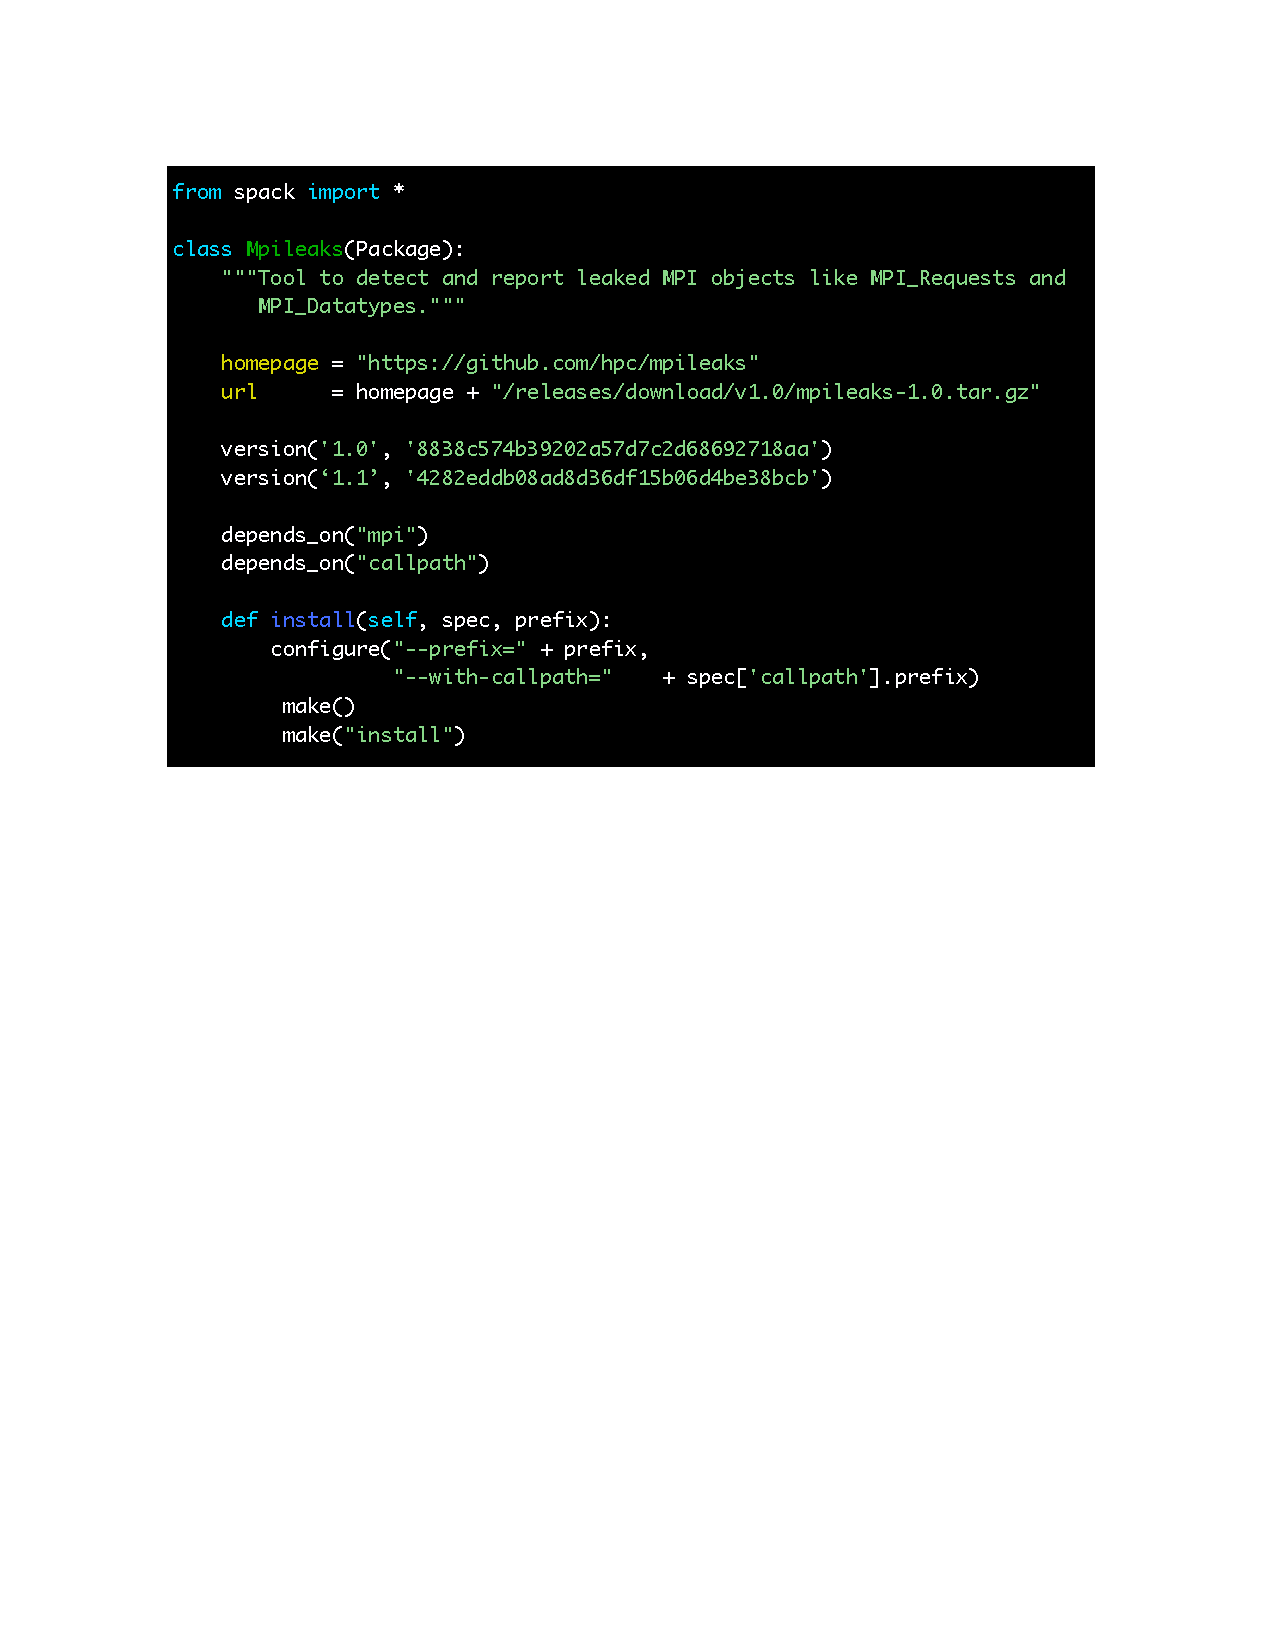
\includegraphics[width=\columnwidth]{code/mpileaks.pdf}
	\caption{
		Spack package for the {\tt mpileaks} tool.
		\label{fig:mpileaks}
	}
\end{figure}

In Spack, packages are build scripts that describe how to build software
artifacts.  Each package is a class written in pure Python to describe
{\it specific} build instructions, and it must extend the {\tt Package}
base class, which implements the more general parts of the build process.
Spack implements a simple, embedded domain-specific language (DSL) to make
packaging easier; it adds special directives such as {\tt depends\_on} and
{\tt version} that add metadata to the class.

Figure~\ref{fig:mpileaks} shows the package for \mpileaks, an LLNL-developed
tool for finding leaks in MPI programs.
Inside the {\tt MpiLeaks} class, the package provides a text description
and a homepage, as well as 
a download URL.  Next, two {\tt version} directives identify known versions
of the package, and MD5 checksums ensure they can be downloaded safely.
Below this, two {\tt depends\_on}
directives indicate prerequisites that must be installed before \mpileaks.
Last, each package defines an {\tt install()} method, which contains the
commands used to build the package.  Spack's DSL allows shell
commands to be invoked as Python functions. Here, the {\tt install()} 
method invokes the familiar {\tt configure}, {\tt make}, and
{\tt make install} build commands, as a shell script would.





